% sections/simulation.tex -- design, methods, declaration, then results
\section{A simulation study of modelling frameworks}\label{sec:simulation}

\subsection{Aims and design}\label{sec:simdesign}

The simulation asks a narrow question: when the true biological response to MHW exposure is lagged and mildly non linear, and the data have the site by year panel structure typical of fisheries monitoring, how well do the modelling frameworks found in the literature recover the exposure effect, and how reliable are the uncertainty statements they produce? Aims, data generating mechanism, estimands, methods and performance measures were fixed in advance \citep{morrisgao2021}, and the implementation is deposited in full (Section~\ref{sec:software}). Table~\ref{tab:design} summarises the design.

\begin{table}[H]
\centering
\caption{Factorial design of the simulation. Exposure depends only on region, grid size, spatial range and replicate, so each of the \nPanels{} unique exposure panels is computed once and reused across the nine combinations of effect size and lag.}
\label{tab:design}
\small
\begin{tabular}{p{6.6cm}p{7.2cm}r}
\toprule
Factor & Levels & $n$ \\
\midrule
Region (real OISST series) & Western Australia; Northwest Atlantic; Mediterranean & 3 \\
True effect $\beta_1$ (per $^{\circ}$C day of lagged cumulative intensity) & $-0.04$; $-0.08$; $-0.12$ & 3 \\
True response lag $L$ (years) & 0; 1; 2 & 3 \\
Spatial correlation range of site noise (km) & 0 (independent sites); 50 & 2 \\
Grid size (sites, 25 km spacing) & 9 ($3 \times 3$); 25 ($5 \times 5$) & 2 \\
\midrule
Scenarios & & \nScenarios{} \\
Replicates per scenario & & \nReplicates{} \\
Unique exposure panels & & \nPanels{} \\
Simulated datasets & & \nDatasets{} \\
Model classes & naive GLM; lag-1 GLM; GAM; DLNM; sdmTMB; random forest & 6 \\
Years per dataset (training / held out) & 41 (38 / 3) & \\
\bottomrule
\end{tabular}
\end{table}

\paragraph{Sea surface temperature.}
Rather than simulate temperature, the study uses three real daily NOAA OISST v2.1 series \citep{banzon2016} bundled with the heatwaveR package \citep{schlegel2018}: the Western Australian shelf, the Northwest Atlantic and the Mediterranean, each spanning 1982 to 2022 (14,975 days). Real series carry the seasonality, autocorrelation, warming trend and pulse statistics that make MHW exposure difficult to model, and they are available to anyone with the package installed.

\paragraph{Event detection and exposure.}
MHWs were detected with heatwaveR using the \citet{hobday2016} defaults: a 1983 to 2012 climatology, the 90th percentile threshold with a 31 day smoothing window, a five day minimum duration and a two day maximum gap for joining events. Figure~\ref{fig:events} shows the detection on each series around its most intense event. On the Western Australian series the canonical algorithm identifies the 2011 event from 6 February to 6 April (\waDur{} days), with maximum intensity \waMax{}\,$^{\circ}$C above climatology and cumulative intensity \waCum{}\,$^{\circ}$C days; it is the most intense event in the series by peak anomaly, although a longer 1999 event exceeds it on the cumulative metric (the full series with every detected event is shown in Online Resource 1, Fig.~S4). These values are regenerated by a verification script on the analyst's machine and stored as the reference against which the test suite checks, because detection output can shift between package versions. The sensitivity of the 2011 event to three climatology windows and two percentile thresholds is reported in Online Resource 1, Table S5. Annual exposure per site was summarised as cumulative intensity above threshold ($i_{\mathrm{cum}}$, $^{\circ}$C days), maximum and mean positive anomaly, days above threshold, event count and onset day.

\begin{figure}[H]\centering
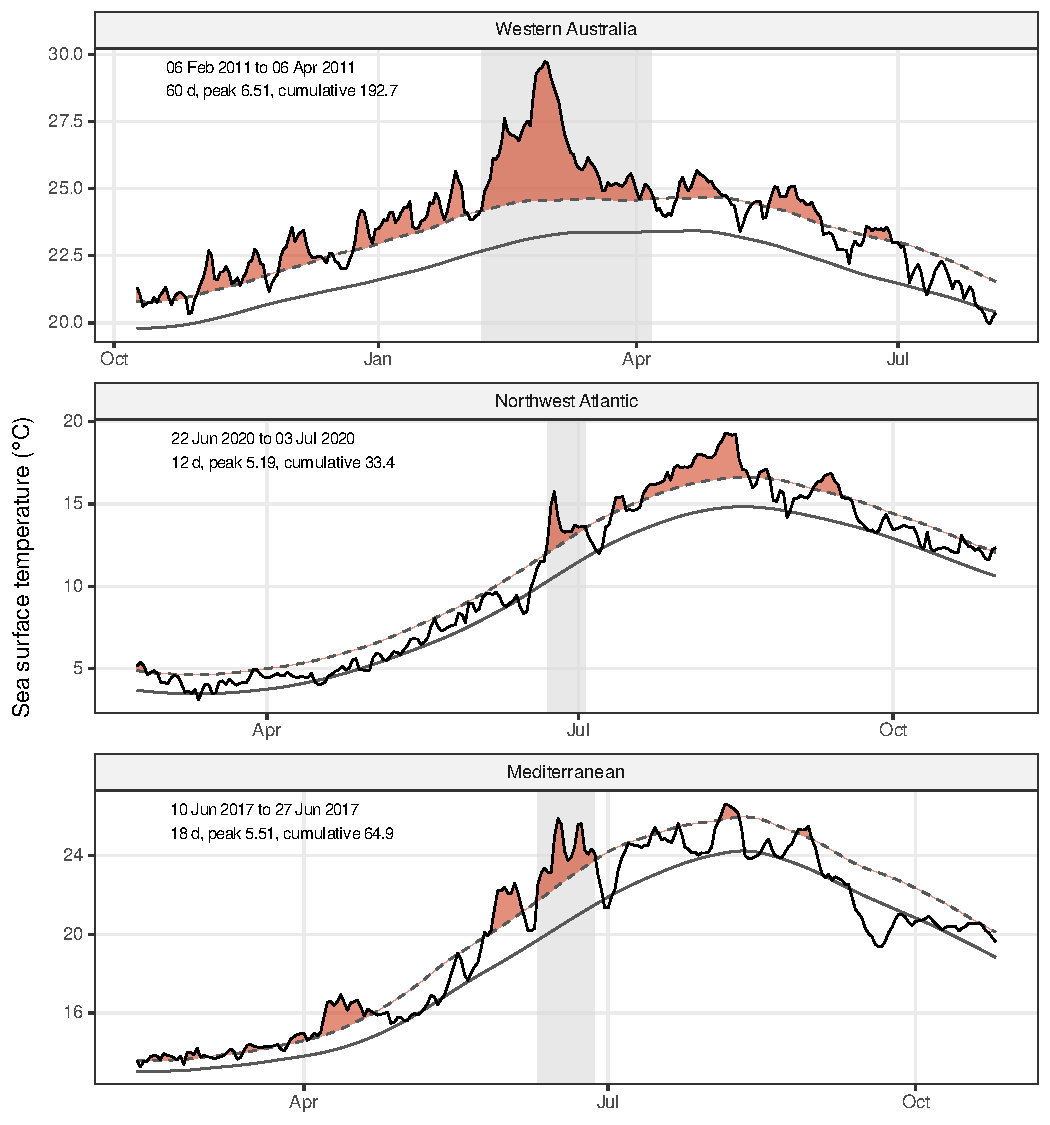
\includegraphics[width=0.92\textwidth]{fig_detection_events}
\caption{Marine heatwave detection on the three real OISST series used in the simulation, each shown for 120 days either side of its most intense event by peak anomaly. Black, daily sea surface temperature; solid grey, seasonal climatology; dashed grey, 90th percentile threshold; shaded, exceedance above threshold; grey band, the detected event with its start, end, duration, peak intensity ($^{\circ}$C) and cumulative intensity ($^{\circ}$C days). Values are as computed by heatwaveR \heatwaveRVersion{} with the Hobday et al. (2016) defaults.}
\label{fig:events}
\end{figure}

\paragraph{Spatial panels.}
Each region's series was replicated across a square grid of sites 25 km apart, with 9 or 25 sites, and a daily noise field with standard deviation 0.3\,$^{\circ}$C was added. The noise was either independent across sites or correlated with an exponential (Mat\'ern $\nu = 1/2$) covariance of range 50 km. Every site therefore shares the real regional trajectory while differing in the timing and magnitude of individual exceedances. Detection and exposure summaries were computed separately for every site.

\paragraph{Data generating process.}
Counts $y_{s,t}$ for site $s$ and year $t$ were drawn from a negative binomial distribution with mean $\mu_{s,t}$ and dispersion $k = 4$, where
\begin{equation}
\log \mu_{s,t} = \alpha + \beta_1 z_{s,t-L} + \beta_2 z_{s,t-L}^{2} + \varepsilon_{s,t}, \qquad \varepsilon_{s,t} = \rho\,\varepsilon_{s,t-1} + \eta_{s,t},
\label{eq:dgp}
\end{equation}
$z$ is $i_{\mathrm{cum}}$ in $^{\circ}$C days, $L$ is the true response lag in years, $\alpha = 2.5$, $\beta_2 = -5 \times 10^{-4}$, $\rho = 0.4$ and the innovations $\eta$ give $\varepsilon$ a stationary standard deviation of 0.3. The quadratic term is small relative to $\beta_1$ but not zero; it represents the saturating behaviour that thermal performance curves imply \citep{sinclair2016} and that linear specifications cannot absorb. With $\alpha = 2.5$ and the observed exposure distributions, mean counts fell between 3 and 7 and the proportion of zeros between 26\% and 44\% across all design cells (Online Resource 1, Table S6), so no cell produced a degenerate response. The response contains no latent spatial field of its own: the only spatial structure is the correlation among site exposure series, which matters for how the spatial model's results are read (Section~\ref{sec:sdmtmb}).

\paragraph{Why lags of zero, one and two years.}
The lag levels follow from the annual cadence of the response and from the response timings documented in the reviewed studies. A lag of zero represents responses that unfold within the year of the event, such as mortality and displacement of adults during the 2011 Western Australian event \citep{caputi2016,yang2019}. A lag of one year represents settlement and recruitment mediated responses, in which the cohort spawned during the event determines the following year's index: the near failure of the 2015 walleye pollock year class \citep{rogers2021} and post settlement cod abundance in the Gulf of Alaska \citep{abookire2022,almeida2024} are of this kind. A lag of two years represents impacts that reach the fished or surveyed age classes only after propagating through recruitment, as in the multi year regulation dynamics of Roe's abalone after 2011 \citep{hart2018}. Longer lags are plausible for long lived species, but with 38 training years and a distributed lag cross basis that already spans lags 0 to 3, lags beyond two cannot be separated from the autocorrelation of exposure itself with any precision. The lag set is a single vector in the configuration file and can be extended by readers whose species warrant it.

\subsection{Models and performance measures}\label{sec:simmodels}

Six model classes were fitted to every dataset (Table~\ref{tab:models}); all were fitted to the first 38 years of each panel with the final three years held out. Table~\ref{tab:models} also gives the estimand each class reports for $\beta_1$. The GLMs and sdmTMB report the coefficient directly. For the GAM it was obtained as the ordinary least squares slope of the fitted smooth over the central 90\% of the exposure range; for the DLNM, as the cumulative log rate ratio at an exposure of 10\,$^{\circ}$C days divided by 10; for the random forest, as the change in mean log prediction when lagged exposure is increased by one unit. These are commensurate only when the response is linear, and their divergence under curvature is part of what the study measures.

\begin{table}[H]
\centering
\caption{Model classes fitted in the simulation, the R implementation used, and the quantity each reports as the estimate of $\beta_1$. NB, negative binomial; GLM, generalised linear model; GAM, generalised additive model; DLNM, distributed lag non linear model; SPDE, stochastic partial differential equation; AR1, first order autoregressive.}
\label{tab:models}
\small
\begin{tabular}{p{2.4cm}p{5.6cm}p{2.4cm}p{3.6cm}}
\toprule
Class & Specification & Package & Estimate of $\beta_1$ \\
\midrule
Naive NB GLM & $y \sim i_{\mathrm{cum},t}$ + site fixed effects; the dominant approach in the reviewed literature & MASS \citep{venables2002} & Coefficient on contemporaneous exposure \\
Lag-1 NB GLM & $y \sim i_{\mathrm{cum},t-1}$ + site fixed effects & MASS & Coefficient on one year lagged exposure \\
NB GAM & $y \sim s(i_{\mathrm{cum},t-1}, k = 6)$ + site random effect, REML & mgcv \citep{wood2017} & OLS slope of the fitted smooth over the central 90\% of exposure \\
DLNM & Cross basis over lags 0 to 3 (natural splines; 3 df exposure, 2 df lag) + site fixed effects, quasi Poisson & dlnm \citep{gasparrini2011} & Cumulative log rate ratio at exposure 10 divided by 10 \\
sdmTMB & $y \sim i_{\mathrm{cum},t-1}$ + Mat\'ern SPDE spatial field + AR1 spatiotemporal field, NB2, 25 km mesh cutoff & sdmTMB \citep{anderson2022,lindgren2011} & Fixed effect coefficient \\
Random forest & $y \sim i_{\mathrm{cum},t}, i_{\mathrm{cum},t-1}$, days above threshold, coordinates; 300 trees & ranger \citep{wright2017} & Finite difference in mean log prediction per unit lagged exposure \\
\bottomrule
\end{tabular}
\end{table}

Performance measures were bias, root mean squared error, empirical coverage of nominal 95\% intervals where an interval is defined, the mean negative binomial log predictive density of the held out years, residual Moran's $I$ of site mean residuals using four nearest neighbours, convergence as judged by each package's own diagnostics (sdmTMB's \texttt{sanity()} function for the spatial model, the iteration limit flags of \texttt{glm.nb} for the GLMs), and wall clock time. Fits that triggered a package warning were retained and recorded as not converged rather than discarded, so that the convergence rates reported are not inflated by silent omission. All summaries were computed across replicates within scenario, then across scenarios.

\subsection{Software, reproducibility and use of generative AI}\label{sec:software}

Every step, from detection through aggregation, figure generation and the tables and numbers in this article, is implemented in R \citep[version \rVersion{};][]{rcore2024} with heatwaveR \heatwaveRVersion{}, dlnm \dlnmVersion{}, mgcv \mgcvVersion{}, sdmTMB \sdmtmbVersion{} and ranger \rangerVersion{}, and released as a tested repository (Data availability). A verification script regenerates the detection reference values on the user's machine and the test suite checks against that file rather than against hard coded numbers. Panel level checkpointing allows the design to be run on a workstation or as a scheduler array job and resumed after interruption; array scripts for SLURM and PBS are included. Every number quoted in Sections~\ref{sec:results} to \ref{sec:discussion} is a macro generated from the deposited output tables.

Generative AI (Claude, Anthropic) was used during preparation of this manuscript for drafting and restructuring code, for drafting prose that was subsequently revised, and for formatting. All code was executed by the author in the environment described above; every numerical result reported here was produced by that execution and reproduced from the deposited outputs before entering the text. The author takes full responsibility for the content.

% sections/results.tex -- every number is a macro from results.tex
\subsection{Results}\label{sec:results}

The five faster model classes were fitted to all \nDatasets{} datasets (\nFitsMain{} fits); the GLMs, GAM, DLNM and random forest returned a point estimate for \glmPctEstimate{}\% of fits, and the small remainder are recorded in the run report (Online Resource 1, Table S12) rather than silently dropped. The sdmTMB model, whose fitting time on spatially independent panels was two orders of magnitude longer than the other classes, was run on \sdmtmbPanelsN{} panels covering \sdmtmbScenarioFrac{} of scenarios (\sdmtmbFits{} fits, \sdmtmbReplicates{} replicates); its results are reported separately in Section~\ref{sec:sdmtmb}. Table~\ref{tab:performance} and Figures~\ref{fig:bias} to \ref{fig:infpred} give the breakdown by model class and lag; Online Resource 1 (Tables S7 to S12) gives every further cut. The text concentrates on the four patterns with consequences for practice.

\performanceTable

\subsubsection{Omitting the lag erases the effect}\label{sec:res-lag}

Figure~\ref{fig:bias} shows the distribution of mean bias in $\hat\beta_1$ across scenarios, by model class and true lag. When the true response was contemporaneous, the naive GLM carried a bias of \naiveBiasLagZero{}, the curvature induced bias that every linear in exposure model conditioning on the correct lag shares (Section~\ref{sec:res-coverage}). When the true lag was one year its bias changed sign and rose to \naiveBiasLagOne{}, and at two years to \naiveBiasLagTwo{}. Against true effects of $-0.04$ to $-0.12$, these biases correspond to under estimation of the effect magnitude by \naiveRelBiasLagOne{}\% at a one year lag and \naiveRelBiasLagTwo{}\% at two years (Fig.~\ref{fig:relbias}). The estimate does not become noisy; it becomes a precise estimate of a much smaller number. In an applied study it would read as a weak or absent effect, with a narrow confidence interval to match.

\begin{figure}[H]\centering
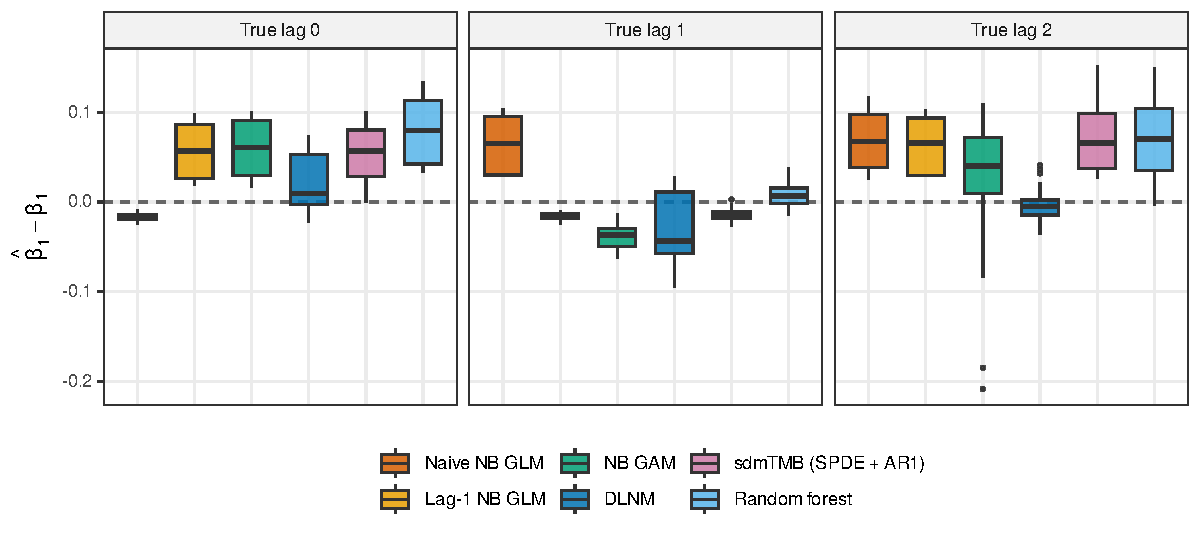
\includegraphics[width=\textwidth]{fig_bias_by_lag}
\caption{Mean bias of the estimated exposure coefficient, $\hat\beta_1 - \beta_1$, across the \nScenarios{} scenarios, by model class and true response lag. Each box summarises one third of the scenarios. The dashed line marks zero bias. Colours identify model classes and are used consistently in all figures.}
\label{fig:bias}
\end{figure}
\begin{figure}[H]\centering
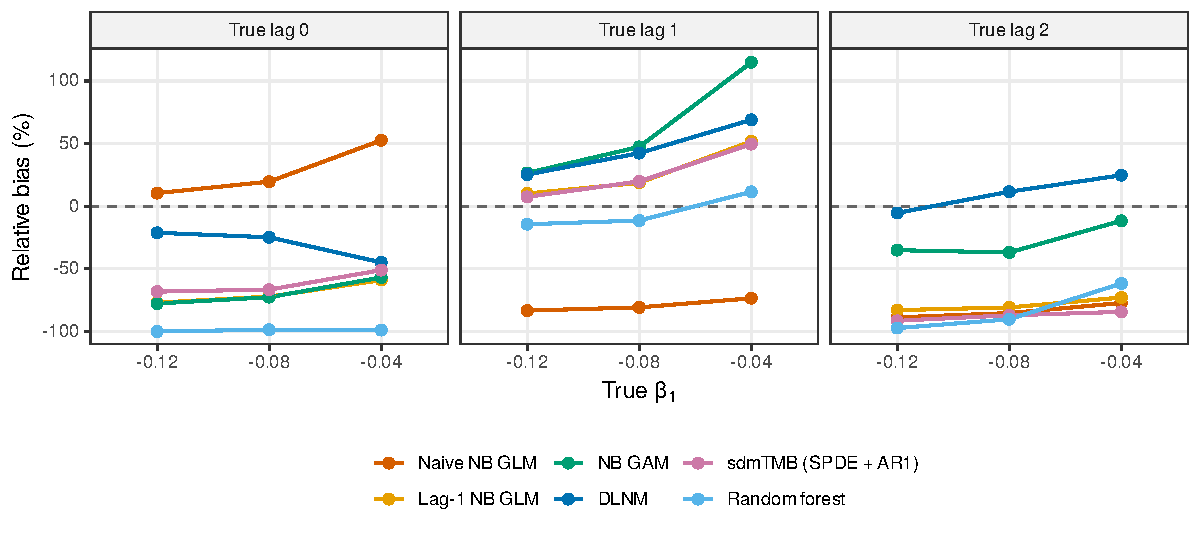
\includegraphics[width=\textwidth]{fig_relative_bias}
\caption{Relative bias, $100(\hat\beta_1-\beta_1)/\beta_1$, by true effect size and true lag. Negative values indicate under estimation of the magnitude of a negative effect.}
\label{fig:relbias}
\end{figure}

The lag aware GLM corrected the problem only when its assumed lag was the true one. At a one year lag its bias was \lagoneBiasLagOne{} (\lagoneRelBiasLagOne{}\% relative), but at zero and two years it collapsed in the same way as the naive model, under estimating by \lagoneRelBiasWrongLag{} respectively. Specifying a lag is therefore not a safeguard unless the lag is known, which in the reviewed literature it rarely was. The GAM, which also conditions on one year lagged exposure, showed the same dependence on the assumed lag.

The distributed lag model behaved differently. Because it estimates the lag profile rather than assuming it, its bias did not switch sign or magnitude with the true lag: \dlnmBiasLagZero{}, \dlnmBiasLagOne{} and \dlnmBiasLagTwo{} at lags of zero, one and two years, with relative bias between \dlnmRelBiasLagZero{}\% and \dlnmRelBiasLagOne{}\%. That robustness came at a cost in precision. The across replicate standard deviation of its estimate at a one year lag was \dlnmSdLagOne{}, against \lagoneSdLagOne{} for the correctly lagged GLM, and its RMSE at that lag (\dlnmRmseLagOne{}) exceeded the correctly lagged GLM's (\lagoneRmseLagOne{}). The practical trade is between an estimator that is accurate only if an unverifiable assumption holds and one that is less precise but does not fail when the assumption is wrong.

\subsubsection{Linear models produce confident intervals around the wrong value}\label{sec:res-coverage}

Nominal 95\% intervals from the two linear GLMs covered the true coefficient in \linearCoverageRange{} of scenarios (Fig.~\ref{fig:coverage}). The failure was not confined to the misspecified lag. Even at the correct lag, where the lag aware GLM's bias was only \lagoneBiasLagOne{}, its coverage was \lagoneCoverageCorrectLag{}, because the small bias induced by the unmodelled quadratic term is large relative to a standard error computed from several hundred site years. The intervals are correctly computed for the fitted model; they are centred on an estimate that the model cannot move to the right place. The GAM, which can represent the curvature, reached \gamCoverageLagOne{} coverage at the correct lag but fell to \gamCoverageMin{} when the lag was wrong. The DLNM's coverage ranged from \dlnmCoverageMin{} to \dlnmCoverageMax{} across lags (mean \dlnmCoverage{}), below nominal but an order of magnitude above the linear models. No class achieved nominal coverage in every condition, which argues for reporting the coverage behaviour of the chosen model under simulated conditions resembling the study rather than assuming it.

\begin{figure}[H]\centering
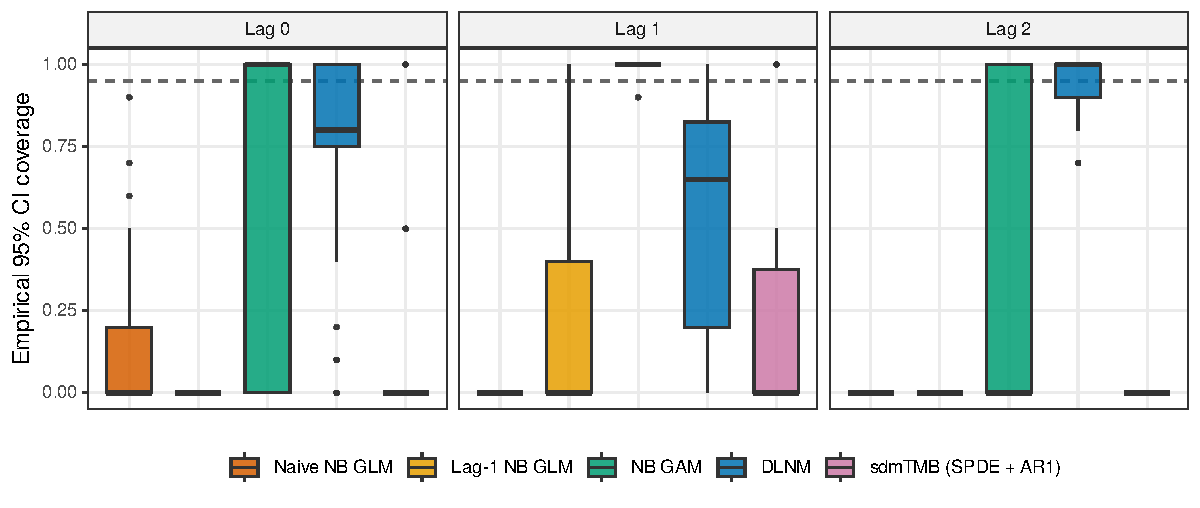
\includegraphics[width=\textwidth]{fig_coverage}
\caption{Empirical coverage of nominal 95\% confidence intervals for $\beta_1$, by model class and true lag. The dashed line marks nominal coverage. The random forest returns no interval and is omitted.}
\label{fig:coverage}
\end{figure}

\subsubsection{The best estimator is not the best predictor}\label{sec:res-prediction}

Held out predictive performance ordered the models differently from coefficient recovery (Fig.~\ref{fig:infpred}). Averaged across all scenarios the naive GLM, with the worst coefficient recovery at non zero lags, produced the highest held out log score (\naiveLogScore{}), followed by the random forest (\rfLogScore{}), the lag aware GLM (\lagoneLogScore{}) and the GAM (\gamLogScore{}). The ordering is driven by the contemporaneous scenarios, where the naive model is correctly specified and predicts well (\naiveLsLagZero{} against \lagoneLsLagZero{} for the lag aware GLM); at a one year lag the lag aware GLM and the GAM predicted better (\lagoneLsLagOne{} and \gamLsLagOne{} against \naiveLsLagOne{}). The random forest, which returns no interpretable coefficient, predicted competitively at every lag and its finite difference effect at a one year lag was nearly unbiased (\rfBiasLagOne{}), although without an interval. The quasi Poisson DLNM has no proper predictive density and was excluded from this comparison. A study that reports a single model cannot show both properties, and the model that would be chosen for prediction is not the one that would be chosen for attribution.

\begin{figure}[H]\centering
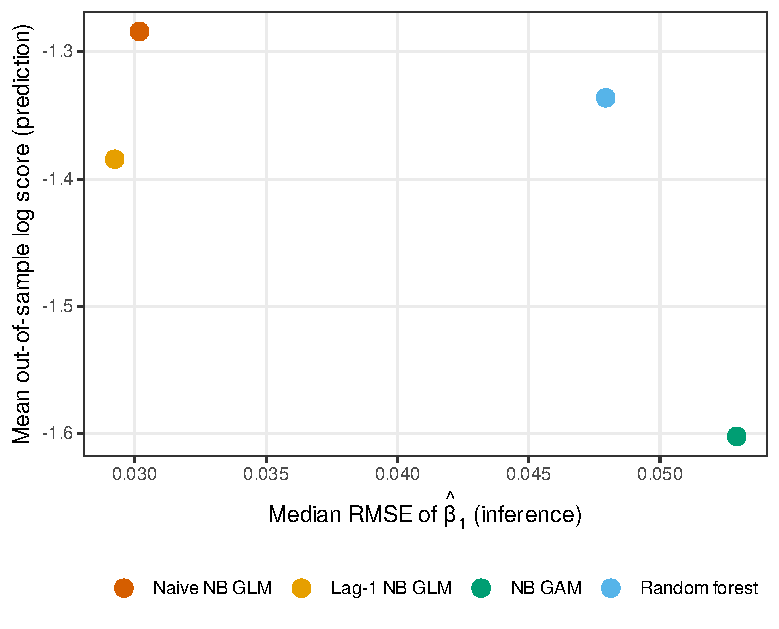
\includegraphics[width=0.6\textwidth]{fig_inference_prediction}
\caption{Coefficient recovery (median RMSE of $\hat\beta_1$ across scenarios) against held out predictive performance (mean negative binomial log predictive density of the final three years), one point per model class. The distributed lag model has no proper predictive density under the quasi Poisson fit and is omitted.}
\label{fig:infpred}
\end{figure}

\subsubsection{Region, grid size and spatial range do not change the ordering}\label{sec:res-region}

The ranking of model classes by absolute bias at a one year lag was \regionRankInvariant{} across the three regions (Fig.~\ref{fig:region}, Online Resource 1, Table S10). The naive GLM's bias at that lag ranged only from \naiveBiasLagOneRegionRange{} across Western Australia, the Northwest Atlantic and the Mediterranean, despite regional exposure distributions whose means differ by more than a factor of two. Grid size and spatial correlation range had no detectable effect on bias for any class (Online Resource 1, Table S11), which is expected because the fixed effect does not depend on the spatial field and the site fixed effects or random effects absorb the correlated noise. Residual Moran's $I$ of site mean residuals was small and negative for all regression classes (\moransIndep{} on independent panels and \moransCorr{} on correlated panels, averaged over models; Online Resource 1, Fig.~S6), confirming that in this design the spatial structure in exposure does not leave residual spatial dependence that a spatial random field would be needed to absorb. The lag problem is therefore not a regional artefact, and it is not alleviated by more sites.

\begin{figure}[H]\centering
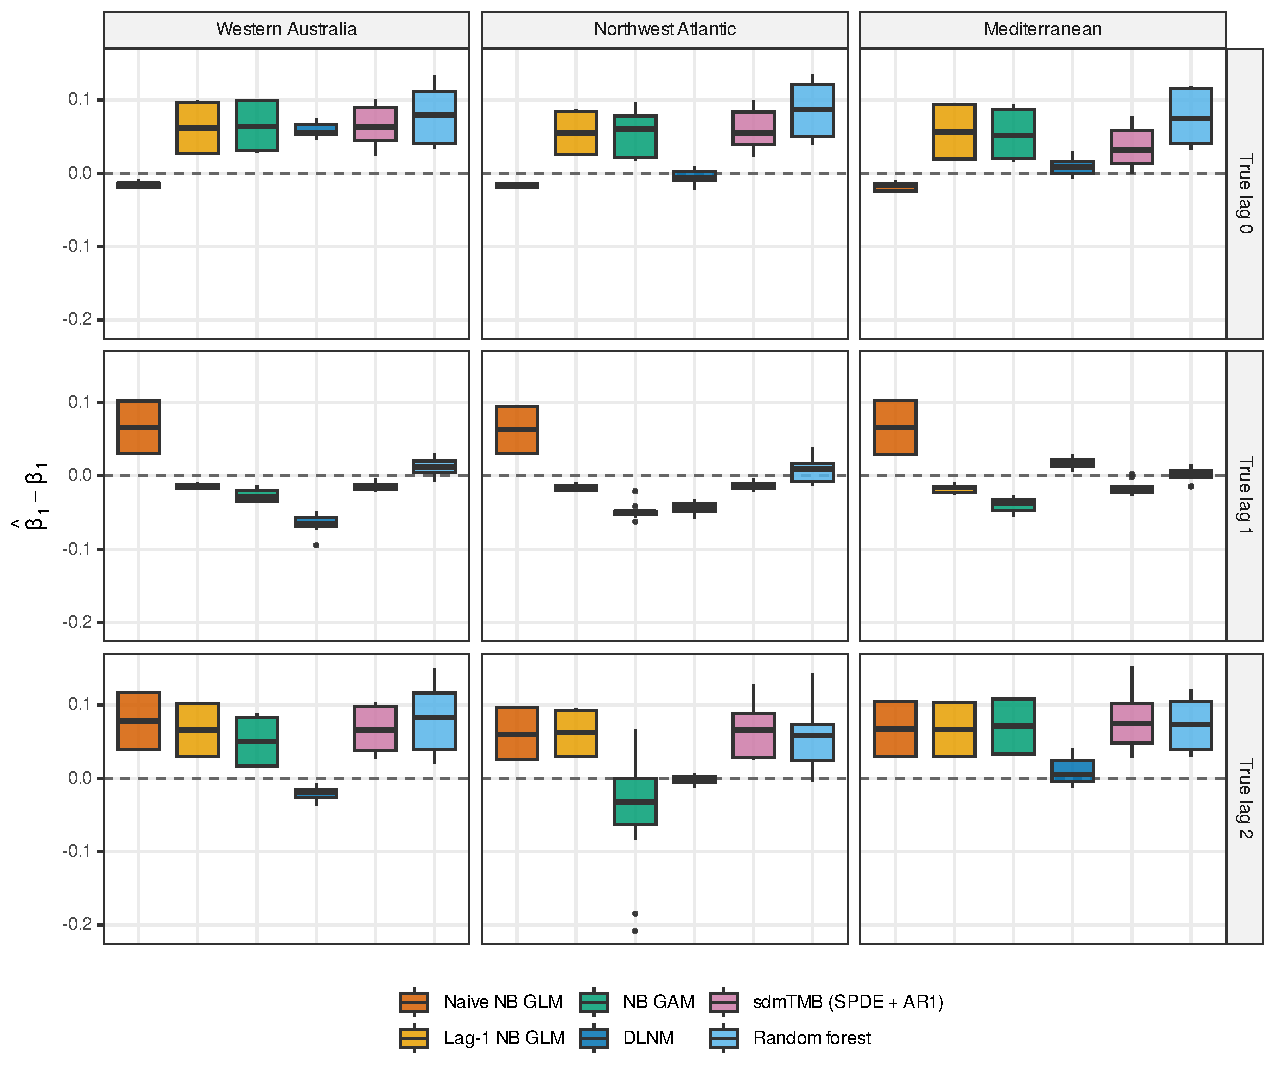
\includegraphics[width=\textwidth]{fig_region}
\caption{Mean bias of the estimated exposure coefficient by region, model class and true lag.}
\label{fig:region}
\end{figure}

\subsubsection{The spatial random field model}\label{sec:sdmtmb}

On the \sdmtmbPanelsN{} panels completed (\sdmtmbFits{} fits), sdmTMB returned point estimates whose bias (\sdmtmbBiasLagZero{}, \sdmtmbBiasLagOne{} and \sdmtmbBiasLagTwo{} at lags of zero, one and two years) tracked the lag aware GLM, as expected for a model that conditions on the same one year lagged covariate. Its \texttt{sanity()} diagnostic flagged \sdmtmbNonConvPct{}\% of fits, most often for a non positive definite Hessian (\sdmtmbNonConvIndep{}\% on spatially independent panels, \sdmtmbNonConvCorr{}\% on correlated ones), and interval coverage was \sdmtmbCoverage{}. These outcomes follow from the design rather than from a defect in the model. Equation~\ref{eq:dgp} contains no latent spatial field in the response; the only spatial structure is correlation among the site exposure series, and the site effects in the fixed effect models absorb it, as the near zero residual Moran's $I$ confirms. sdmTMB is therefore estimating a spatial variance and a spatiotemporal variance that are both truly zero, which places the optimiser at a boundary and is exactly the condition under which the package's documentation warns that the Hessian will be flagged. The design can show that a spatial random field model does not rescue a mis specified lag structure, and that its diagnostics report the absence of a field honestly; it cannot show the conditions under which such a model recovers a spatially varying effect, which would require a different data generating process (Section~\ref{sec:discussion}). Median fitting time was \sdmtmbMedianSec{}\,s per fit, against \naiveSec{}\,s for the GLM, which is the practical reason the model was run on a subset of the design.

